\documentclass[crop,tikz]{standalone}
\usepackage{graphicx} % Required for inserting images
\usepackage{tikz}
\tikzstyle{block} = [rectangle, minimum width=2cm, minimum height=1cm,text centered, draw=black]
\tikzstyle{block_1} = [rectangle, minimum width=2cm, minimum height=1cm,text centered, draw=black, fill=blue!5]
\tikzstyle{block_2} = [rectangle, minimum width=2cm, minimum height=1cm,text centered, draw=black, fill=red!5]
\tikzstyle{arrow} = [thick,->,>=stealth]
\tikzstyle{arrow_2} = [very thick,->,>=stealth]
\tikzstyle{arrow_3} = [thick,->,>=stealth,dashed]
\tikzstyle{pfr} = [cylinder, draw, minimum height=4cm, minimum width=1cm, shape aspect=1, shape border rotate=180]
\usetikzlibrary{shapes.geometric}

\begin{document}
\begin{center}
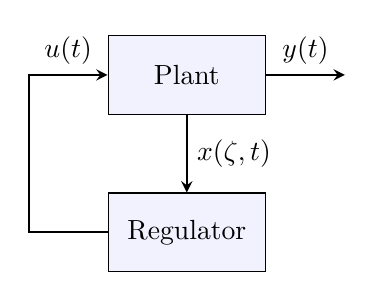
\begin{tikzpicture}[node distance=2cm]
    \node (plant) [block_1] {Plant};
    \node (regulator) [block_1, below of=plant] {Regulator};
    \draw [arrow] (plant.south) -- node[midway, right] {$x(\zeta,t)$} (regulator.north);
    \draw [arrow] (regulator.west) -- ++(-1,0) |- node[near end, above] {$u(t)$} (plant.west);
    \draw [arrow] (plant.east) -- node[midway, above] {$y(t)$} ++(1,0);
\end{tikzpicture} 
\end{center}
\begin{center}
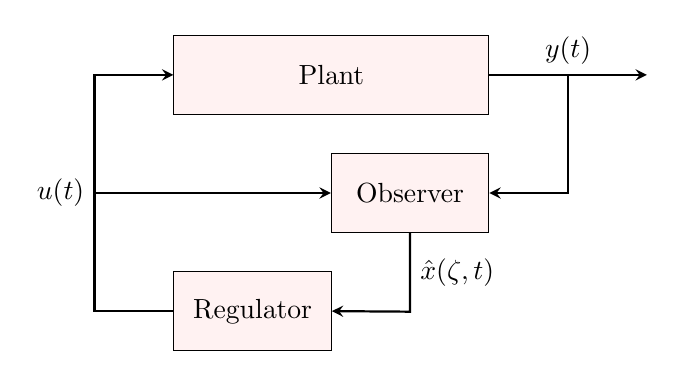
\begin{tikzpicture}[node distance=2cm]
    \node (plant) [block_2, minimum width=4cm] {Plant};
    \node (regulator) [block_2, below of=plant, xshift=-1cm, yshift=-1cm] {Regulator};
    \node (observer) [block_2, below of=plant, xshift=1cm, yshift=0.5cm] {Observer};
    \draw [arrow] (plant.east) -- node[midway, above] {$y(t)$} ++(2,0);
    \draw [arrow] (plant.east) ++(1,0) |- (observer.east);
    \draw [arrow] (observer.south) -- ++(0,-1) node[midway, right] {$\hat{x}(\zeta,t)$} -- (regulator.east);    
    \draw [arrow] (regulator.west) -- ++(-1,0) |- (plant.west);
    \draw [arrow] (regulator.west) ++(-1,1.5) coordinate(start) -- node[near start, left, xshift=-0.75cm] {$u(t)$} (observer.west);
\end{tikzpicture} 
\end{center}
\begin{center}
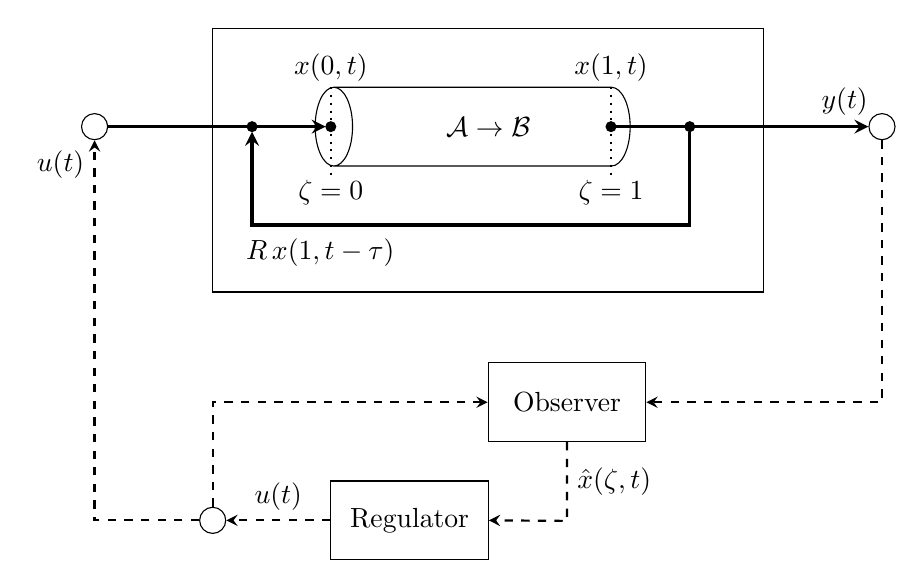
\begin{tikzpicture}
    \draw (-3.5,-2.1) rectangle (3.5,1.25);
    \node (pfr) [pfr] {$\mathcal{A} \rightarrow \mathcal{B}$};
    \node (regulator) [block, below of=pfr, xshift=-1cm, yshift=-4cm] {Regulator};
    \node (observer) [block, below of=pfr, xshift=1cm, yshift=-2.5cm] {Observer};
    \node (pfr_output) [circle, right of=pfr, xshift=4cm, draw, minimum size=0.25cm] {};
    \node (pfr_input) [circle, left of=pfr, xshift=-4cm, draw, minimum size=0.25cm] {};
    \node (obsv_input) [circle, left of=regulator, xshift=-1.5cm, draw, minimum size=0.25cm] {};
    \node (pfr_inlet) [circle, left of=pfr, xshift=-1cm, fill=black, draw, inner sep=0pt, minimum size=0.25cm, scale=0.5] {};
    \node (pfr_outlet) [circle, at={(pfr.east)}, shift={(-0.25cm,0)}, fill=black, draw, inner sep=0pt, minimum size=0.25cm, scale=0.5] {};
    \node (recycle_right) [circle, right of=pfr_outlet, fill=black, draw, inner sep=0pt, minimum size=0.25cm, scale=0.5] {};
    \node (recycle_left) [circle, left of=pfr_inlet, fill=black, draw, inner sep=0pt, minimum size=0.25cm, scale=0.5] {};

    \draw[dotted, thick] ([yshift=0.5cm]pfr_inlet.center) -- node[at end, below, yshift=0.1cm] {$\zeta = 0$} ([yshift=-0.65cm]pfr_inlet.center);
    \draw[dotted, thick] ([yshift=0.5cm]pfr_outlet.center) -- node[at end, below, yshift=0.1cm] {$\zeta = 1$} ([yshift=-0.65cm]pfr_outlet.center);

    \node[below of=recycle_left, node distance=1.3cm, anchor=north west, xshift=-0.2cm] {$R \, x(1, t-\tau)$};
    \node[above of=pfr_inlet, node distance=0.75cm,] {$x(0, t)$};
    \node[above of=pfr_outlet, node distance=0.75cm,] {$x(1, t)$};
    
    \draw [arrow_2] (pfr_outlet) -- node[near end, above, xshift=0.5cm] {$y(t)$} (pfr_output);
    \draw [arrow_2] (pfr_input.east) -- (pfr_inlet);
    \draw [arrow_2] (recycle_right) -- ++(0,-1.25) -| (recycle_left);
    
    \draw [arrow_3] (pfr_output) |- (observer.east);
    \draw [arrow_3] (observer.south) -- ++(0,-1) node[midway, right] {$\hat{x}(\zeta,t)$} -- (regulator.east); 
    \draw [arrow_3] (regulator.west) -- node[midway, above] {$u(t)$} (obsv_input.east);
    \draw [arrow_3] (obsv_input.west) -| node[at end, below left] {$u(t)$} (pfr_input.south);
    \draw [arrow_3] (obsv_input.north) |- (observer.west);
\end{tikzpicture}
\end{center}

\begin{center}
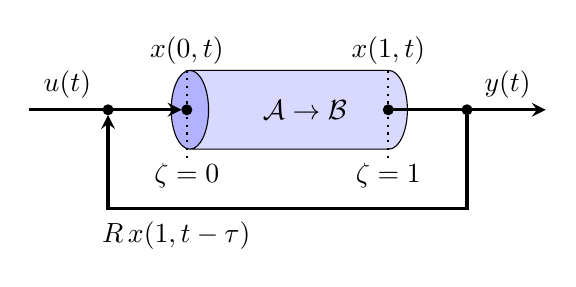
\begin{tikzpicture}
    \node (pfr) [cylinder, draw, minimum height=3cm, minimum width=1cm, shape aspect=1, shape border rotate=180, cylinder uses custom fill, cylinder end fill=blue!30, cylinder body fill=blue!15] {$\mathcal{A} \rightarrow \mathcal{B}$};
    \node (pfr_inlet) [circle, left of=pfr, xshift=-0.5cm, fill=black, draw, inner sep=0pt, minimum size=0.25cm, scale=0.5] {};
    \node (pfr_outlet) [circle, at={(pfr.east)}, shift={(-0.25cm,0)}, fill=black, draw, inner sep=0pt, minimum size=0.25cm, scale=0.5] {};
    \node (recycle_right) [circle, right of=pfr_outlet, fill=black, draw, inner sep=0pt, minimum size=0.25cm, scale=0.5] {};
    \node (recycle_left) [circle, left of=pfr_inlet, fill=black, draw, inner sep=0pt, minimum size=0.25cm, scale=0.5] {};

    \draw[dotted, thick] ([yshift=0.5cm]pfr_inlet.center) -- node[at end, below, yshift=0.1cm] {$\zeta = 0$} ([yshift=-0.65cm]pfr_inlet.center);
    \draw[dotted, thick] ([yshift=0.5cm]pfr_outlet.center) -- node[at end, below, yshift=0.1cm] {$\zeta = 1$} ([yshift=-0.65cm]pfr_outlet.center);

    \node[below of=recycle_left, node distance=1.3cm, anchor=north west, xshift=-0.2cm] {$R \, x(1, t-\tau)$};
    \node[above of=pfr_inlet, node distance=0.75cm,] {$x(0, t)$};
    \node[above of=pfr_outlet, node distance=0.75cm,] {$x(1, t)$};
    
    \draw [arrow_2] (pfr_outlet) -- node[near end, above] {$y(t)$} ++(2,0);
    \draw [arrow_2] (pfr_inlet) ++(-2,0) coordinate(start) -- node[near start, above] {$u(t)$} (pfr_inlet);
    \draw [arrow_2] (recycle_right) -- ++(0,-1.25) -| (recycle_left);
    
\end{tikzpicture}
\end{center}
\end{document}
